% 新增格式為:
% \normalsize \item "標題" \par
%     \tiny \input{"檔案在Jc11-codebook底下的完整路徑"}

% Notice:
% 因為中文會造成字型縮小,可以的話"標題"請盡量用英文

\begin{enumerate}
    \normalsize \item Most Divisor Number \par
        \tiny \begin{tabular}[c]{|l|r|r|}
    \hline
    Range & 最多因數數 & 因數個數 \\
    \hline
    $10^9$ & $735134400$ & $1344$ \\
    $2^{31}$ & $2095133040$ & $1600$ \\
    $10^{18}$ & $897612484786617600$ & $103680$ \\
    $2^{64}$ & $9200527969062830400$ & $161280$ \\
    \hline
\end{tabular}
    \normalsize \item Catlan Number \par
        \tiny \[ C_n=\frac{1}{n}\binom{2n}{n}, C_{n+1}=\frac{2(2n+1)}{n+2}C_n \] \par
\[C = 1, 1, 2, 5, 14, 42, 132, 429, 1430, 4862, ... \]

    \normalsize \item Faulhaber's formula \par
        \tiny \[ \sum_{k=1}^{n} k^p = \frac{1}{p+1} \sum_{r=0}^{p} \binom{p+1}{r} B_rn^{p-r+1} \]
\[ \text{where} \ B_0 = 1, \ B_r = 1-\sum_{i=0}^{r-1} \binom{r}{i} \frac{B_i}{r-i+1} \]
也可用高斯消去法找$deg(p+1)$的多項式,例:
\[ \sum_{k=1}^{n} k^2 = a_3n^3 + a_2n^2 + a_1n + a_0 \]
\tiny\[
    \begin{bmatrix}
        0^3 & 0^2 & 0^1 & 0^0\\
        1^3 & 1^2 & 1^1 & 1^0\\
        2^3 & 2^2 & 2^1 & 2^0\\
        3^3 & 3^2 & 3^1 & 3^0
    \end{bmatrix}
    \begin{bmatrix}
        a_3 \\ a_2 \\ a_1 \\ a_0
    \end{bmatrix} =
    \begin{bmatrix}
        0^2 \\ 0^2+1^2 \\ 0^2+1^2+2^2 \\ 0^2+1^2+2^2+3^2
    \end{bmatrix}
\]
\tiny\[
    \begin{bmatrix}
        0 & 0 & 0 & 1 & 0 \\
        1 & 1 & 1 & 1 & 1 \\
        8 & 4 & 2 & 1 & 5 \\
        27 & 9 & 3 & 1 & 14
    \end{bmatrix}
    \Rightarrow \begin{bmatrix}
        1 & 1 & 1 & 1 & 1 \\
        0 & 4 & 6 & 7 & 3 \\
        0 & 0 & 6 & 11 & 1 \\
        0 & 0 & 0 & 1 & 0
    \end{bmatrix}
\]
\[ 
    A = \begin{bmatrix}
        1/3 \\ 1/2 \\ 1/6 \\ 0 
    \end{bmatrix}, \ 
    \sum_{k=1}^{n} k^2 = \frac{1}{3}n^3 + \frac{1}{2}n^2 + \frac{1}{6}n
\]
    \normalsize \item SG Function \par
        \tiny {\raggedright
    \( SG(x) = mex\{SG(y)|x\rightarrow y\} \) \par
    \( mex(S) = min\{n|n\in\mathbb{N}, n\notin S\} \) \par
}
    \normalsize \item Fibonacci \par
        \tiny \[
      \begin{array}{l}
            \begin{bmatrix} f_{n-1} & f_n \end{bmatrix}
            \begin{bmatrix} 0 & 1 \\ 1 & 1 \end{bmatrix} =
            \begin{bmatrix} f_n & f_{n+1} \end{bmatrix} \\
            \begin{bmatrix} f_n & f_{n+1} \end{bmatrix}
            {\begin{bmatrix} 0 & 1 \\ 1 & 1 \end{bmatrix}}^p =
            \begin{bmatrix} f_{n+p} & f_{n+p+1} \end{bmatrix},
            p \in \mathbb{N}
      \end{array} 
\]
\[
      F_n = \frac{1}{\sqrt{5}} \left [ \left( \frac{1+\sqrt{5}}{2} \right)^n- \left( \frac{1-\sqrt{5}}{2} \right)^n \right ] 
\]
    \normalsize \item Pick's Theorem \par
        \tiny 給定頂點座標均是整點(或正方形格子點)的簡單多邊形,其面積$A$和內部格點數目$i$、邊上格點數目$b$的關係為
\normalsize \[ A=i+\frac{b}{2}-1 \]

    \normalsize \item Euler's Formula \par
        \tiny 對於有$V$個點、$E$條邊、$F$個面(含外部)的連通平面圖
\normalsize \[ F+V-E=2 \]
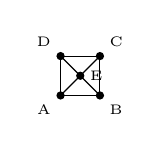
\begin{tikzpicture}         % Graph 1
    % 定義頂點的位置
    \coordinate (A) at (0, 0);
    \coordinate (B) at (0.5, 0);
    \coordinate (C) at (0.5, 0.5);
    \coordinate (D) at (0, 0.5);
    \coordinate (E) at (0.25, 0.25);
    
    % 畫出頂點
    \fill (A) circle (1.5pt) node[below left, font=\tiny] {A};
    \fill (B) circle (1.5pt) node[below right, font=\tiny] {B};
    \fill (C) circle (1.5pt) node[above right, font=\tiny] {C};
    \fill (D) circle (1.5pt) node[above left, font=\tiny] {D};
    \fill (E) circle (1.5pt) node[right, font=\tiny] {E};
    
    % 畫出邊
    \draw (A) -- (B);
    \draw (A) -- (D);
    \draw (A) -- (E);
    \draw (B) -- (C);
    \draw (B) -- (E);
    \draw (C) -- (D);
    \draw (C) -- (E);
    \draw (D) -- (E);
\end{tikzpicture}
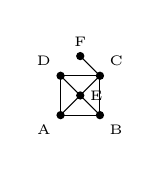
\begin{tikzpicture}         % Graph 2
    % 定義頂點的位置
    \coordinate (A) at (0, 0);
    \coordinate (B) at (0.5, 0);
    \coordinate (C) at (0.5, 0.5);
    \coordinate (D) at (0, 0.5);
    \coordinate (E) at (0.25, 0.25);
    \coordinate (F) at (0.25, 0.75);
    
    % 畫出頂點
    \fill (A) circle (1.5pt) node[below left, font=\tiny] {A};
    \fill (B) circle (1.5pt) node[below right, font=\tiny] {B};
    \fill (C) circle (1.5pt) node[above right, font=\tiny] {C};
    \fill (D) circle (1.5pt) node[above left, font=\tiny] {D};
    \fill (E) circle (1.5pt) node[right, font=\tiny] {E};
    \fill (F) circle (1.5pt) node[above, font=\tiny] {F};
    
    % 畫出邊
    \draw (A) -- (B);
    \draw (A) -- (D);
    \draw (A) -- (E);
    \draw (B) -- (C);
    \draw (B) -- (E);
    \draw (C) -- (D);
    \draw (C) -- (E);
    \draw (C) -- (F);
    \draw (D) -- (E);
\end{tikzpicture}
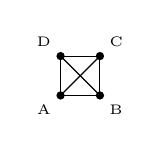
\begin{tikzpicture}         % Graph 3
    % 定義頂點的位置
    \coordinate (A) at (0, 0);
    \coordinate (B) at (0.5, 0);
    \coordinate (C) at (0.5, 0.5);
    \coordinate (D) at (0, 0.5);
    
    % 畫出頂點
    \fill (A) circle (1.5pt) node[below left, font=\tiny] {A};
    \fill (B) circle (1.5pt) node[below right, font=\tiny] {B};
    \fill (C) circle (1.5pt) node[above right, font=\tiny] {C};
    \fill (D) circle (1.5pt) node[above left, font=\tiny] {D};
    
    % 畫出邊
    \draw (A) -- (B);
    \draw (A) -- (C);
    \draw (A) -- (D);
    \draw (B) -- (C);
    \draw (B) -- (D);
    \draw (C) -- (D);
\end{tikzpicture}
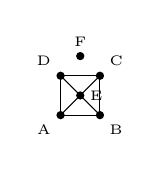
\begin{tikzpicture}         % Graph 4
    % 定義頂點的位置
    \coordinate (A) at (0, 0);
    \coordinate (B) at (0.5, 0);
    \coordinate (C) at (0.5, 0.5);
    \coordinate (D) at (0, 0.5);
    \coordinate (E) at (0.25, 0.25);
    \coordinate (F) at (0.25, 0.75);
    
    % 畫出頂點
    \fill (A) circle (1.5pt) node[below left, font=\tiny] {A};
    \fill (B) circle (1.5pt) node[below right, font=\tiny] {B};
    \fill (C) circle (1.5pt) node[above right, font=\tiny] {C};
    \fill (D) circle (1.5pt) node[above left, font=\tiny] {D};
    \fill (E) circle (1.5pt) node[right, font=\tiny] {E};
    \fill (F) circle (1.5pt) node[above, font=\tiny] {F};
    
    % 畫出邊
    \draw (A) -- (B);
    \draw (A) -- (D);
    \draw (A) -- (E);
    \draw (B) -- (C);
    \draw (B) -- (E);
    \draw (C) -- (D);
    \draw (C) -- (E);
    \draw (D) -- (E);
\end{tikzpicture}
\begin{tiny}
    (1)、(2)正確;(3)$\overline{AC}$與$\overline{BD}$相交,錯誤;(4)非連通圖
\end{tiny}
\end{enumerate}